Large language models (LLMs) achieve remarkable performance across domains such as mathematics, science, and law~\citep{AlphaProof2024_DMind,guha2023legalbench,saab2024capabilities}, in part because they can store vast amounts of knowledge in their parameters~\citep{petroni2019language,meng2023locatingeditingfactualassociations}.
Prior work suggests that knowledge in Transformers is stored in Multi-Layer Perceptrons (MLPs) as key-value mappings, or \emph{facts}~\citep{geva2021transformerfeedforwardlayerskeyvalue,dai2022knowledgeneuronspretrainedtransformers}.
However, despite these findings, fact-storing MLPs remain poorly understood.

While prior work has made important progress toward understanding and modeling fact storage in MLPs, existing models fail to capture three empirically observed properties of LLM fact storage: MLPs must (i) attain optimal fact storage scaling, (ii) handle arbitrary input/output geometries, and (iii) work inside Transformers.
Mechanistic interpretability work~\citep{geva2021transformerfeedforwardlayerskeyvalue,dai2022knowledgeneuronspretrainedtransformers} assumes MLPs store facts in individual neurons, but these models lead to suboptimal storage-capacity scaling.
More recently, \citet{nichani2024understandingfactualrecalltransformers} study LLM fact storage by introducing an MLP \emph{weight construction} (NTK MLP) with theoretical capacity guarantees.
However, existing constructions
(i) theoretically and empirically do not attain the empirically observed information-theoretically optimal capacity scaling of LLMs;
(ii) are restricted to isotropic (e.g., uniformly spherical) embedding distributions, whereas LLM embeddings are anisotropic \citep{ethayarajh2019contextualcontextualizedwordrepresentations,razzhigaev2024shapelearninganisotropyintrinsic}; and 
(iii) cannot be used by Transformer blocks for factual recall tasks, such as answering ``What is the capital of France?''.

Our core insight is to study MLP decoding margin scaling (\Cref{def:margin}). Where prior works focus on fact-storage under noiseless key queries, our decoding margin study allows us to develop the first closed-form MLP construction that is usable by Transformers for factual recall. Consequently, we theoretically show that \emph{Transformer blocks are capable of information-theoretically optimal fact storage} -- providing the first theoretical explanation that aligns with the empirical capacity scaling observed in pretrained LLMs.

Our construction is the first to capture all three empirically observed properties of LLM fact storage:
\begin{figure}[t]
    \centering
    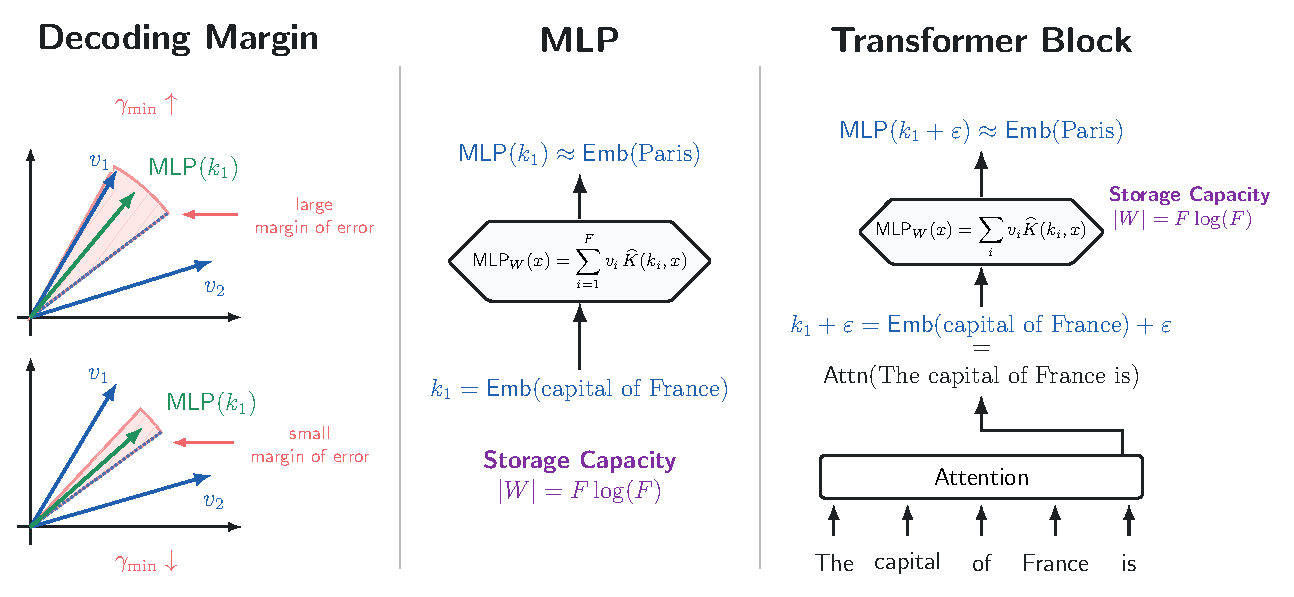
\includegraphics[
        width=\linewidth,
    ]{sections/section_1_intro/figs/banner_fig.pdf}
    \caption{
    \textbf{(A) Decoding margin illustration:} Top plot shows an MLP with large decoding margin, bottom plot with low decoding margin. The MLP with larger decoding margin has a larger ``margin of error'', making it more robust when queried with perturbed versions of $\mathbf{k}_1$. \textbf{(B) MLPs are information-theoretically optimal:} we show that MLPs are Hebbian memories in kernel space and that the storage capacity of MLPs scales at the information-theoretically optimal rate. \textbf{(C) Transformer blocks are information-theoretically optimal:} we show that the storage capacity of Transformer blocks scales at the information-theoretically optimal rate, provided the attention noise remains bounded.
    }
    \label{fig:main-figure}
\end{figure}




\begin{itemize}[leftmargin=1em, itemsep=0.5em]
\item \textbf{Optimal fact-storage capacity and margin (Sections \ref{sec:basic_setting}, \ref{sec:hebbian-kernel-mlps}).}
Our first step toward matching the empirically optimal fact-storage scaling of LLMs is to demonstrate that 1) MLPs are Hebbian kernel memories and 2) that Hebbian kernel memories achieve asymptotically optimal fact-storage scaling. We show this by developing a closed-form MLP construction, equivalent to a Hebbian memory with sketched quadratic kernel, which provably attains a fact storage capacity of $F = \Theta(W / \log W)$ for $F$ facts using $W$ parameters (\cref{cor:optimal-fact-storage-capacity}).
Theoretically, our construction closes the optimality gap over prior constructions by a factor of $\log^{11} F$ under isotropic embeddings.
Moreover, we show that, at matched fact count, the NTK baseline requires $10$-$104\times$ more parameters than our best data-dependent kernel construction (\cref{fig:sketched_k2_sweeps}c).

\item \textbf{Handling arbitrary embedding geometries (\Cref{sec:hebbian-kernel-mlps}).}
We next study how arbitrary embedding geometries affect MLP margin and storage capacity scaling. We show that generalizing the MLP margin and capacity scaling to arbitrary embedding geometries introduces four embedding-geometric statistics multiplicatively into the information-theoretically optimal scaling derived for isotropic embeddings (\cref{thm:bilinear-scaling}). Intuitively, these statistics penalize the margin and capacity scaling by how clustered the key and value embeddings are. Empirically, we show that our generalized bounds characterize the empirical decoding margin scaling precisely ($R^2 \geq 0.95$; \cref{fig:app:beta-sweeps}c). Furthermore, we find that the capacity gap between our construction and trained MLPs is preserved even under anisotropic embeddings.


\item \textbf{MLPs usable within Transformers for factual recall (\Cref{sec:usability}).}
Towards understanding MLP usage within LLMs, we find that non-trivial decoding margin is needed by MLPs to be used for factual recall within Transformer blocks. Attention layers produce imperfect, noisy queries, so the fact-storing MLPs they query should be robust to noise. Building on this insight, we demonstrate theoretically and empirically, for the first time, that Transformer blocks can retrieve facts from MLPs with optimal fact-storage capacity to solve factual recall tasks (\cref{thm:noise-robust-capacity}, \cref{fig:ssfr_main_fig}c). Moreover, in these Transformer experiments, at matched fact count, the NTK baseline requires roughly $15$-$63\times$ more parameters than Transformer blocks using our data-dependent construction.
\end{itemize}

Finally, as a proof-of-concept, we show that fact-storing MLPs enable \emph{modular fact editing} (\Cref{sec:fact-editing}) by replacing a Transformer's MLP with one storing new facts.
Our method, \textsc{MLP Swapping}, achieves near-perfect \emph{fact-editing score}---correctly editing target facts while avoiding off-target effects---whereas prior state-of-the-art methods degrade to as low as $\sim30$\% score when editing 10\% of the fact-set.

In summary, our work takes a constructive step toward understanding MLPs in Transformers. We present a fact-storing MLP construction that achieves optimal margin and fact-storage capacity, provides provable decoding-margin guarantees under arbitrary embeddings, and is usable within Transformer blocks for factual recall at optimal capacity. We also demonstrate an application to modular fact editing, illustrating a path toward robust and modular knowledge manipulation in LLMs.
